\section{Trådløs kommunikation via Bluetooth Low Energy}
\textit{Dette afsnit gennemgår design, implementering og test af systemets trådløse kommunikation mellem de to benyttede MCUer. Disse designes for at kunne lave et trådløst system, hvorefter det implementeres til algoritmerne. Afslutningsvis testes de opstillede krav, som ses i \secref{krav_BLE}}

\subsection{Design}
Systemet vil involvere to MCUer, henholdsvis en GAP central og en GAP peripheral. Begge enheder er påført et BLE modul, således dataoverførslen mellem enhederne foregår ved brug af dette. Denne dataoverførsel mellem MCUerne er illustreret som pseudokode på \figref{fig:blue_pseudo}. 
\begin{figure}[H]
	\centering
	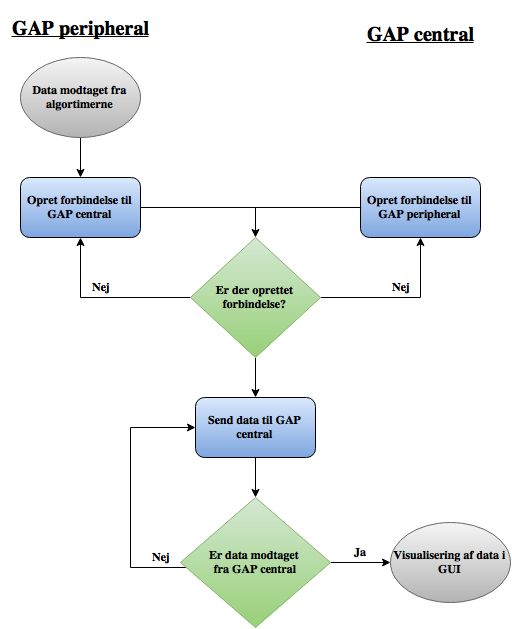
\includegraphics[scale=0.5]{figures/cDesign/blue_pseudo.png}
	\caption{På figuren ses flowchartet for den trådløse kommunikation og dataoverførsel mellem GAP central og GAP peripheral. Indledningsvis forsøges der at oprette forbindelse mellem enhederne, hvorefter dataoverførslen finder sted. Ved fuldendt dataoverførsel bliver BLE modulet for de to enheder sat i dvaletilstand.}
	\label{fig:blue_pseudo}
\end{figure}
Ovenstående pseudokode er bestemmende for, hvorvidt en MCU fungerer som GAP central eller peripheral i et kredsløb. Enheden, som programmeres til GAP central, skal modtage data fra den anden enhed. Ydermere skal GAP central overføre denne data til en computer gennem en USB port, således visualisering i en GUI er muligt. \newline
Førend dataoverførselen er mulig, skal der skabes en forbindelse mellem de to enheder, hvilket ligeledes fremgår af \figref{fig:blue_pseudo}. Hvis ikke dette lykkes, gentages proceduren indtil forbindelsen er oprettet. %Når der er etableret forbindelse mellem enhederne overføres dataene, som modtages fra algoritmerne fra PSoC 4200M. 
Systemet vil ikke fortsætte til næste element i pseudokoden, medmindre dataoverførslen har været succesfuld.  

\subsection{Implementering}
GAP peripheral er den MCU, der er ansvarlig for dataopsamling, signalbehandling og afsendelse af data til GAP central. Opsætningen af MCUerne som henholdsvis GAP central og GAP peripheral udføres i PSoC Creator, hvor Topdesign af EZ-BLE modulerne er afgørende for rollen i kredsen. Standardkoder fra Cypress' hjemmesider benyttes til indstilling af rollen for MCUen. \newline
PSoC 4200M på GAP peripheral konfigureres således, at det færdigbehandlede data vil blive ført mod EZ-BLE modulet. Denne konfiguration udføres ved at initialisere en UART forbindelse imellem de to mikroprocessorer samt indstille designet af pins i PSoC Creater. % de pågældende pins for PSoC 4200M og EZ-BLE i pindesign i PSoC Creator. 
Port P3[0] på GAP peripheral 4200M benyttes til UART:RX og port P3[1] til UART:TX. Ydermere konfigureres EZ-BLE modulet til at benytte P1[4] til UART:RX og port P1[5] til UART:TX. Disse konfigurationer sikrer, at der forekommer en dataoverførsel fra PSoC 4200M og videre til EZ-BLE, hvorfra dataene kan sendes til GAP central. \citep{Semiconductor20164200M} \newline
GAP central skal konfigureres således, at denne kan modtage data og herefter overføre dette til en computer gennem USB porten. I denne konfiguration benyttes ligeledes til 4200M port P3[0] til UART:RX og port P3[1] til UART:TX og til EZ-BLE ligeledes port P1[4] til UART:RX og port P1[5] til UART:TX. 
%Ydermere benyttes port P7[0] til UART:RX og port P7[1] til UART:TX. Dermed er det muligt at overføre datene fra PSoC LP5 til en computer. 
%Det fremgår af \figref{fig:blue_pseudo}, at BLE modulerne skal sættes til en lavere powermode, når dataoverførslen er fuldendt. Derfor vil C kodning af BLE modulerne medvirke til, at denne handling er mulig.

\subsection{Test}
Den trådløse kommunikation BLE testes for at undersøge rækkevidden af denne kommunikation. Testen udføres med henhold til de opstillede krav og tilhørende tilladte afvigelser opstillet i \secref{krav_BLE}. Kravene til den trådløse kommunikation er, at den trådløse kommunikation skal:
\begin{itemize}
	\item Være i stand til at sende data indenfor en rækkevidde på 3 meter. Der accepteres ikke en kortere rækkevidde.
\end{itemize}

I testen undersøges rækkevidden for den trådløse kommunikation ved, at GAP peripheral bliver sat til at videresende datapakker, som GAP central skal modtage alle af. Hvis dataoverførslen er nøjagtig, vil der ikke mangle nogle pakker. Dette vil blive illustreret igennem MATLAB, hvori en nøjagtig overførsel vil medføre en fuldstændig lineær kurve. Hvis datapakker er gået tabt, vil illustrationen af antal modtagne pakker varierer fra antal sendte pakker med stor hældning, og den kurven vil ikke være lineær. Denne test udføres med forskellig afstand mellem GAP peripheral og GAP central, hvoraf den maksimale afstand for succesfuld dataoverførsel vil komme til udtryk. \\
Datapakkerne i denne test sendes fire gange i sekundet, og resultaterne bliver opsamlet igennem 30 sekunder. Der skabes forbindelse mellem GAP peripheral og GAP central, hvor antallet af modtagne datapakker optages igennem RealTerm. Derfra konverteres det fra hex til decimaltal, hvormed data kan plottes i matlab.\fxnote{capture, optaget i hex, konverteret til decimaltal, som er plottet i matlab}
\begin{table}[H]
	\centering
	\begin{tabular}{cc}
			\hline
		\rowcolor[HTML]{C0C0C0} 
		Afstand {[}m{]} & Tabte datapakker \\ 	\hline
		0,5 	& 0\% \\ 	\hline
		1 		& 0\% \\	\hline
		1,5 	& 0\% \\	\hline
		2 		& 0\% \\	\hline
		2,5 	& 0\% \\	\hline
		3 		& 0\% \\	\hline
		3,5 	& 0\% \\	\hline
		4 		& 100\% \\	\hline
	\end{tabular}
	\caption{I tabellen ses sammenhængen mellem antal tabte datapakker omregnet til procent og afstanden mellem GAP peripheral og GAP central.}
	\label{test:ble_overforsel}
\end{table} \vspace{-.5cm}
Testresultaterne i \tabref{test:ble_overforsel} viser, at med en afstand på mere end 3,5 meter kan GAP peripheral og GAP central ikke opretholde kontakten. Dette fremgår ligeledes af \figref{fig:test_ble}, hvor der ses, at antallet af sendte og modtagende pakker har en lineær sammenhæng op til 3,5 meter.
\begin{figure}[H]
	\centering
	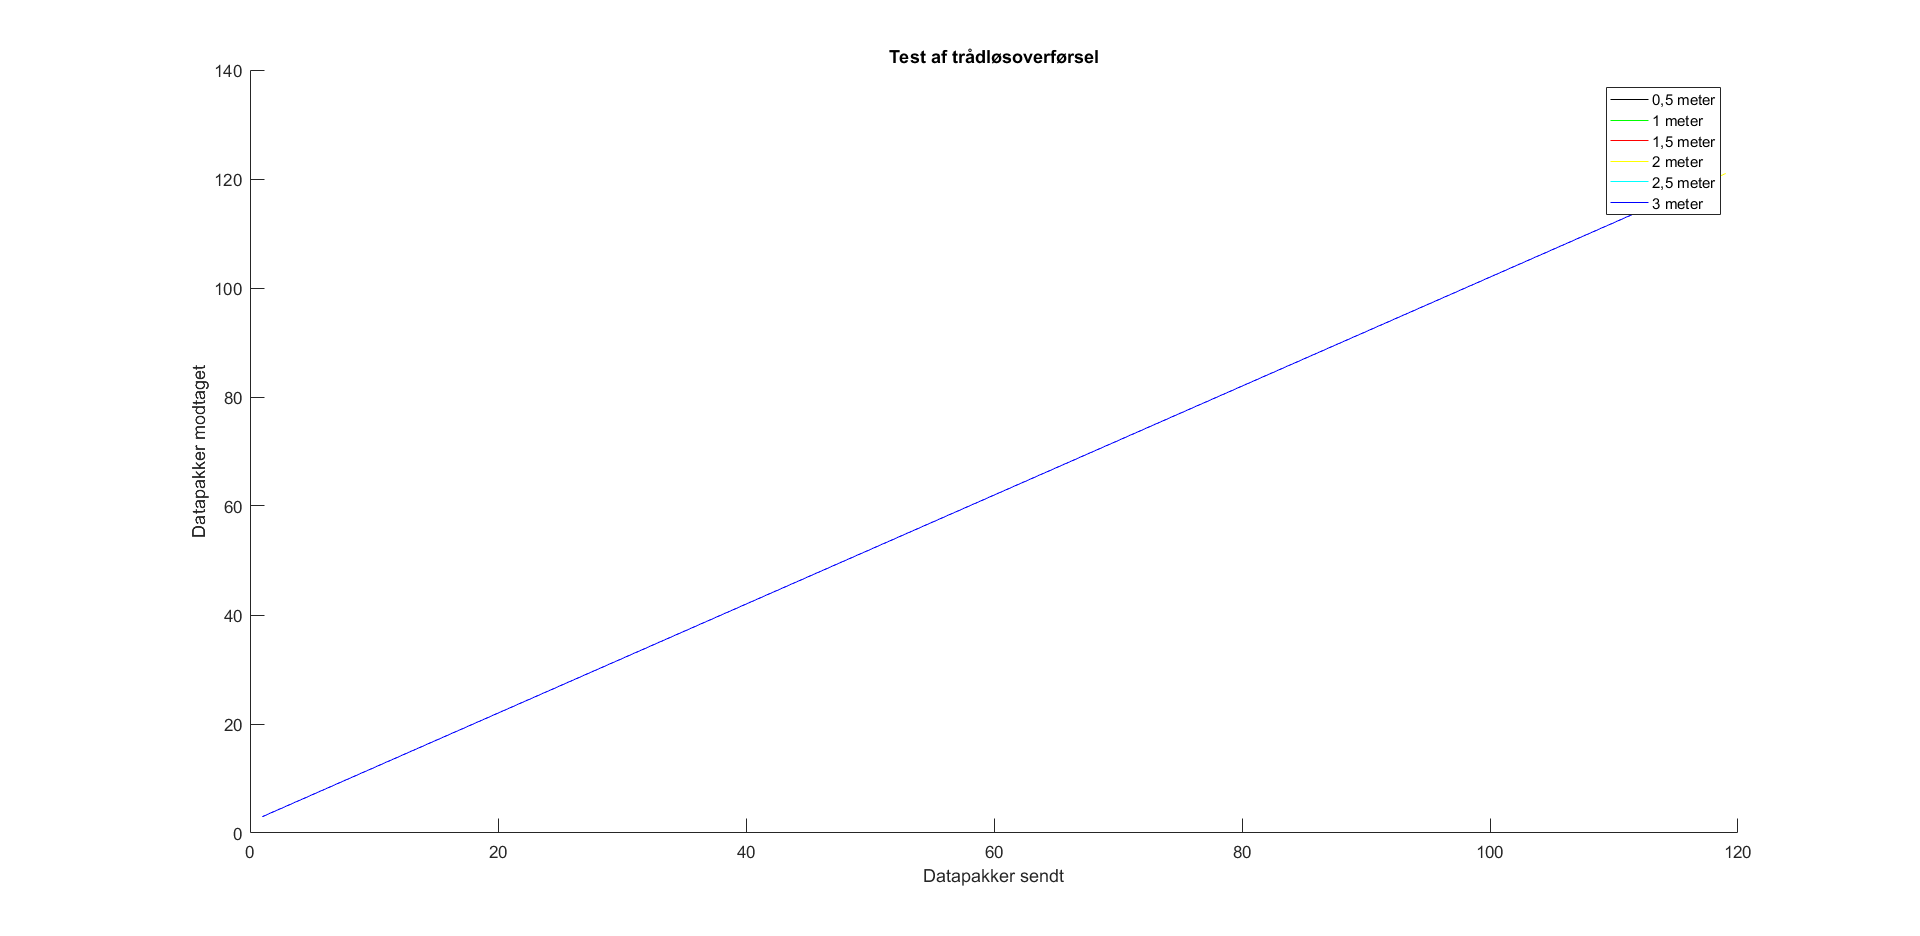
\includegraphics[scale=0.45]{figures/cDesign/test_ble.png}
	\caption{På figuren ses et grafisk plot af forholdet mellem antal sendte pakker sammenholdt med antal modtagne datapakker. }
	\label{fig:test_ble}
\end{figure}
Alle datapakker op til 3,5 meter blev modtaget, hvorfor der ikke forekommer udsalg på \figref{fig:test_ble}. På figuren ses kun den blå kurve, da de andre ligger bag denne, eftersom disse ligeledes ikke har mistet nogle datapakker og ligger på samme linje. Hvis afstanden mellem GAP peripheral og GAP central overskrider 3,5 meter, afbrydes forbindelsen og datapakkerne bliver ikke sendt. \\
Kravet om, at data mellem de to MCUer udelukkende skal sendes med trådløs kommunikation i form af BLE, er dermed muligt at opfylde. Den trådløse kommunikation mellem systemets enheder overholder kravet vedrørende afsendelse og modtagelse af korrekt data inden for 3 meters afstand. Kravet vedrørende tab af data heraf overholdes ligeledes, da datapakker først går tabt over 3,4 meters afstand.
